
\documentclass[a4paper,10pt,notitlepage]{article}

\usepackage{a4wide}
\usepackage{amssymb} 
\usepackage{amsmath} 
%\usepackage{algorithmic} 
%\usepackage{algorithm} 


% Tilpasning til Dansk.
%\usepackage[latin1]{inputenc}
%\usepackage[T1]{fontenc}

\usepackage{graphicx}
\usepackage{colortbl}
\usepackage{url}
\usepackage{listings}


\begin{document}
% Forsiden skal v�re side 1, s� denne side m� v�re nummer 2.
%\addtocounter{page}{1}


\newenvironment{my-itemize}{
   \begin{list}
   {$\bullet$}
   { \addtolength{\leftmargin}{\labelsep}
      \setlength{\topsep}{1ex}
      \setlength{\itemsep}{0ex}
      \setlength{\parsep}{0ex}}
}
{\end{list}}


\newcommand{\myFigure}[3]{
   \begin{figure}[!ht]
      \centering
      \includegraphics[width=#1\textwidth, clip=true]{\cdir #2.png}
   \caption{#3}
   \label{fig:#2}
   \end{figure}
}



\title{{\bf J3DScene: A Java-library for fast and easy visualization of 3D scenes.}}
\author{{Rasmus Fonseca} and {Pawel Winter}}

\maketitle

\begin{abstract}
Creating and displaying 3D scenes containing basic geometric objects is important when discussing, teaching, debugging and developing geometrically related algorithms. Also, displaying molecular structures with user-defined properties (e.g. transparent bounding volumes or color-indications of energy-interactions etc.) will benefit researchers working with problems within structural bioinformatics. J3DScene is a 3D java library for quickly and easily creating, animating and viewing 3D scenes. This tool will aid researchers in visualizing their geometric algorithms, datastructures and problem domains without taking valuable time from research. 
\end{abstract}
\begin{figure}[!ht]
\centering
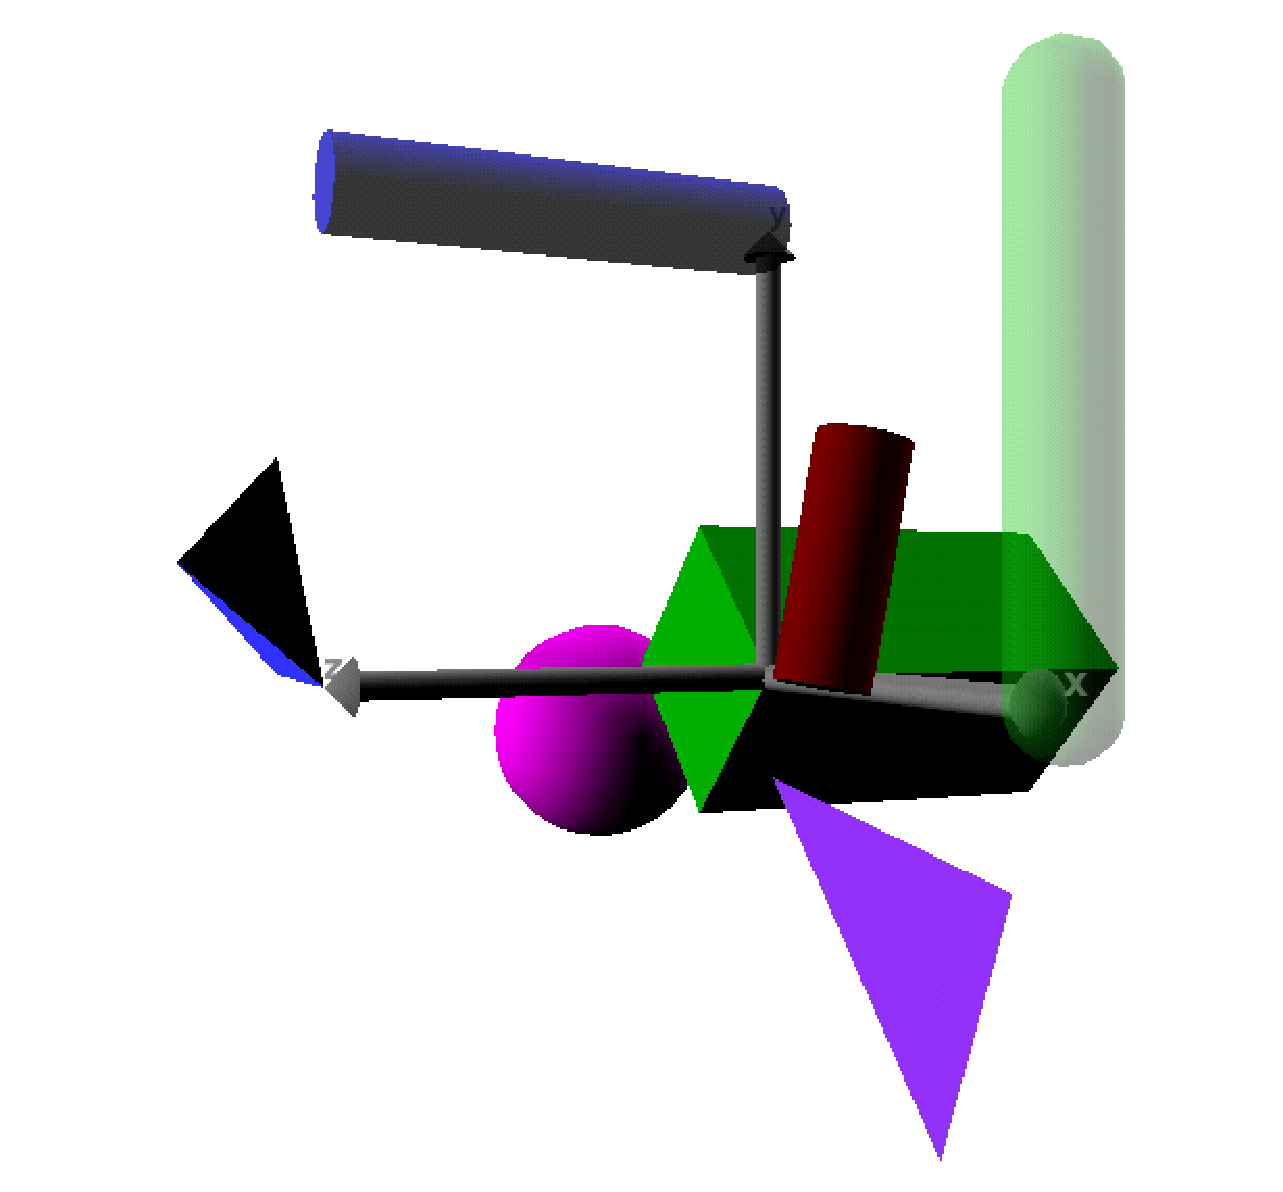
\includegraphics[width=0.6\textwidth]{J3DScene}
\end{figure}

\section{Introduction}

%Motivation and design-goals
% - Java
% - Fast results
% - Simple API / short manual
% - Extendible / modular
A large set of algorithms and problems in computer science are related to 3D objects. Computational geometry, in particular, is the study of algorithms which can be stated in terms of geometry. We have developed a Java library which can visualize geometric objects and assist the study of geometric methods and problems. 
%It is designed with an emphasis on being easy to use and on enabling easy navigation within a 'live' 3D scene. 
It is designed with the following emphases:
\begin{itemize}
\item 3D scenes must be created quickly and with minimum effort from the user. Creating a scene or adding a primitive to the scene requires, at most, two lines of Java code. The use of J3DScene furthermore requires no knowledge of Java3D or the swing-library. 
\item The API to J3DScene is minimal. Each basic primitive has a single class and the scene is represented using a single class with only X methods. 
\item Navigating a scene is easily demonstrated and live. 
\end{itemize}
A 3D scene viewer is considered 'live' if the view can update objects positions and shapes approximately as fast as the human eye can register. This is the only requirement to the efficiency of the library, and is achievable for scenes containing up to roughly X primitives. The reason why a Java library is developed, as opposed to a complete application, is to ease the inclusion in existing Java-based software projects. 

%Existing software
% - Rasmol
% - JMol
% - Blender
% - Povray
% - FPV
% - Java3D
There exists a plethora of different applications and libraries for generating 3D graphics. For viewing molecular structures Rasmol, JMol and FPV are excellent open-source viewers that reads molecular description files (PDB-files) and displays them. Different views, such as protein backbone only or space-fill atoms, can typically be chosen to highlight different important aspects. The geometric primitives used to generate molecular graphics are usually only cylinders (for covalent bonds) and spheres (for atoms). These viewers are only well-suited for their specific purposes, i.e. viewing molecules. Sometimes user-specified properties such as enclosing volumes or color-coded high-energy atom interactions must be illustrated. However, doing this in JMol for instance requires a significant amount of work and knowledge of the extensible code base of JMol. 

For very advanced 3D scene creation blender and povray can be used. Blender is a graphical user interface for creating 3D models, and is a widely used open-source IDE for 3D modeling. Povray has an extensible scene description language and, given a scene specified in a text-file, a ray-traced image can be generated. Any 3D shape can be generated using these applications, but both have a steep learning curve and they use too complicated rendering methods to render 3D scenes live. 

A significant amount of scene-graph-based Java libraries exists, such as Java3D, 3DzzD, Ardor 3D and Xith 3D. These are all general purpose libraries suitable for creating, displaying and navigating live 3D scenes. However, using any of these requires intimate knowledge of scene-graphs which takes significant time to get familiar with. For instance, the introductory chapter of the Java3D manual is 20 pages long. 

\newcommand{\jc}[1]{\textbf{#1}}
\newcommand{\jm}[1]{\textbf{#1}}
\section{Design}
The J3DScene-library is designed using a single central class, \jc{J3DScene}, which encloses all the required 3D functionality (see Figure \ref{fig:classDiagram}). The \jm{addShape}, \jm{removeShape} and \jm{removeAllShapes}-methods are responsible for adding and removing the different shapes to and from the scene. Moving shapes is handled implicitly by changing the fields of the shape, and calling \jm{repaint}. 

\begin{figure}[!ht]
\centering
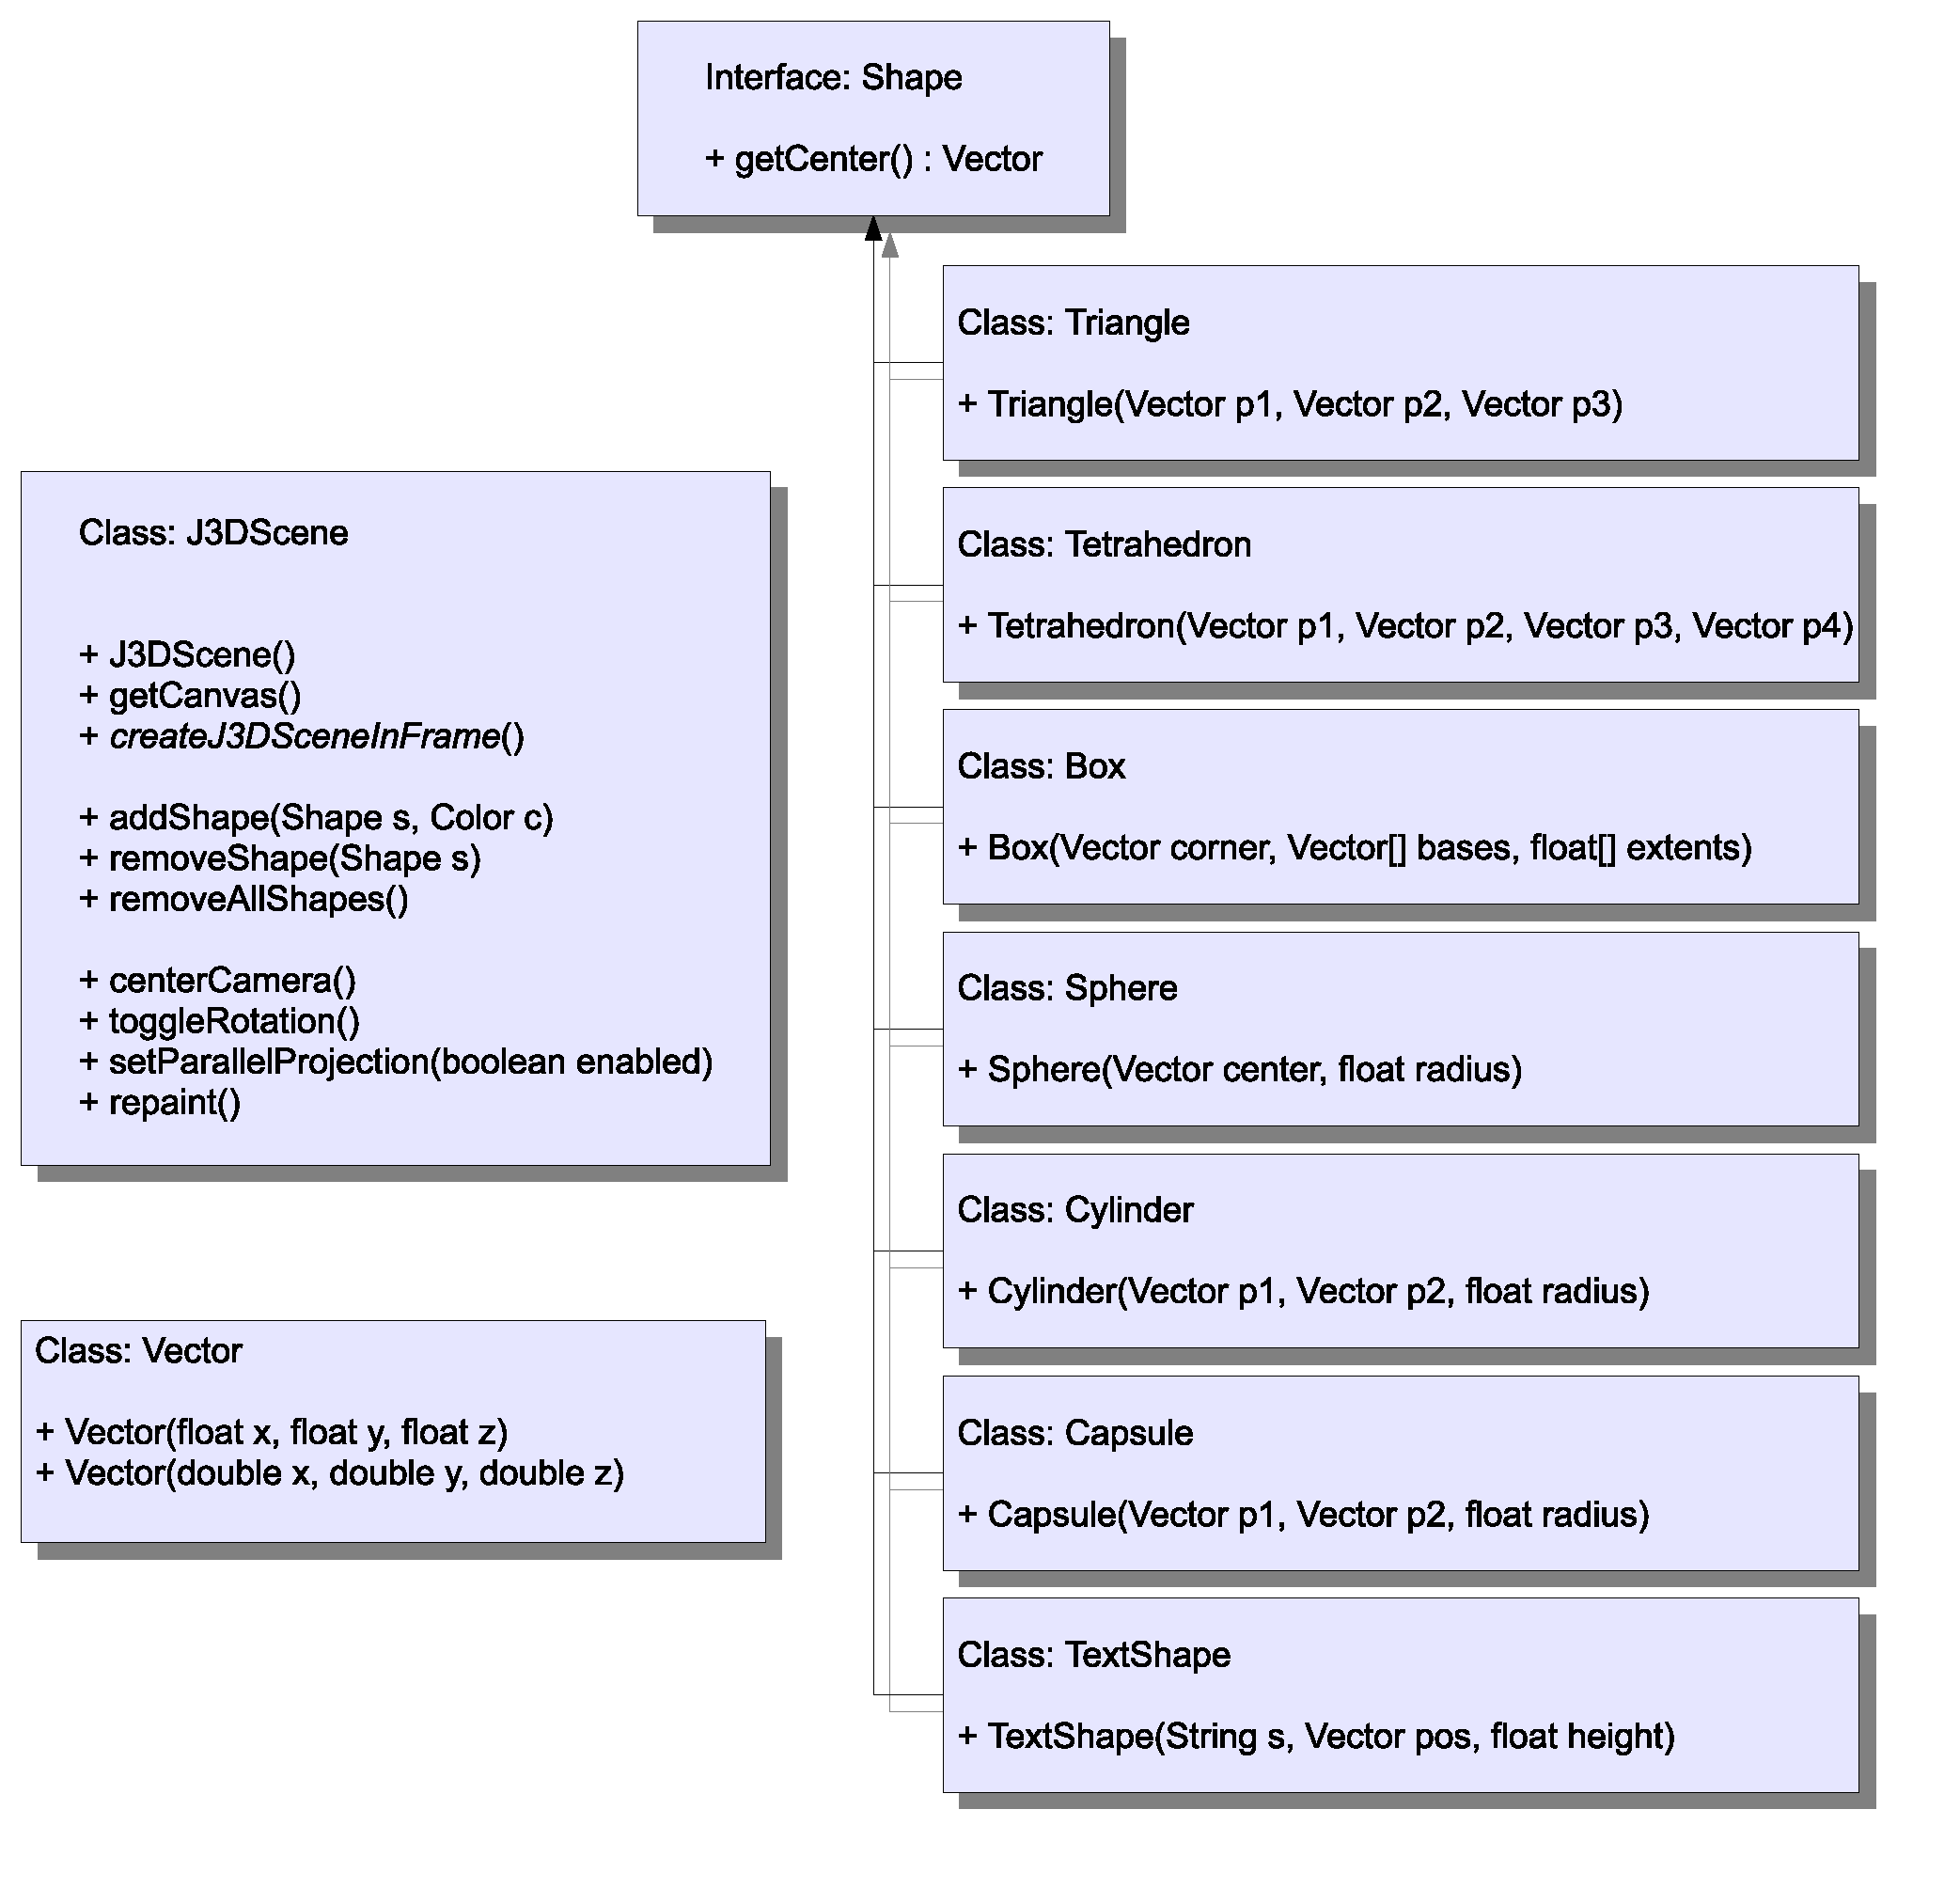
\includegraphics[width=0.8\textwidth]{figures/classDiagram}
\caption{Class-diagram for J3DScene}
\label{fig:classDiagram}
\end{figure}

All 3D shapes must implement the \jc{Shape} interface and be supported by the \jc{J3DScene} class. Most shapes specify a position which is implemented in the \jc{Vector}-class. 



\section{Manual}
%\newenvironment{codepiece}{}{}
\newcommand{\codepiece}[1]{\hspace{0.1\textwidth}\framebox[0.8\textwidth]{#1}}
%Adding shapes
% - Add shapes example (with colors, and transparency).
% - Removing shapes example
% - 
To create a scene displaying a gray ball simply write\\
\rule{\linewidth}{0.2mm}\vspace{0.8mm}
\begin{minipage}[b]{0.7\linewidth}
\scriptsize
\begin{verbatim}
J3DScene scene = J3DScene.createJ3DSceneInFrame();
scene.addShape(new Sphere(new Vector(1,0,0), 0.5f);
\end{verbatim}
\end{minipage}
\begin{minipage}[b]{0.3\linewidth}
Figure
\end{minipage}
\rule{\linewidth}{0.2mm}
The static \jm{createJ3DSceneInFrame} method creates a \jc{JFrame} with a 3D-canvas and returns the scene-object that is painted in that canvas. If, for any reason, one wishes more control of the canvas object the following example illustrates how to create the scene object and use the canvas object

\noindent
\rule{\linewidth}{0.2mm}\vspace{0.8mm}
\begin{minipage}[b]{0.7\linewidth}
\scriptsize
\begin{verbatim}
J3DScene scene = new J3DScene();
scene.addShape(new Sphere(new Vector(1,0,0), 0.5f);

JFrame frame = new JFrame();
frame.setSize(600,600);
frame.getContentPane().add(scene.getCanvas());
frame.setVisible(true);
JPopupMenu.setDefaultLightWeightPopupEnabled(false);
\end{verbatim}
\end{minipage}
\begin{minipage}[b]{0.3\linewidth}
\rule{\linewidth}{0.2mm}\vspace{0.8mm}
Figure
\end{minipage}
\rule{\linewidth}{0.2mm}
It is recommended in ?? to call the \jm{setDefaultLightWeightPopupEnabled} method when using Java3D. 

%Controlling view
% - Mouse controls
% - Keyboard controls

%Advanced features
% - Getting the clicked object. 
% - Storing to image file
% - Animating


\section{Conclusion}


\bibliographystyle{unsrt}
\bibliography{../../BibliographyFile}
\end{document}
